\subsection{Fonctionnement de la diffusion de quiz avec WebSocket}

\vspace{3mm}
\begin{figure}[H]
\centering
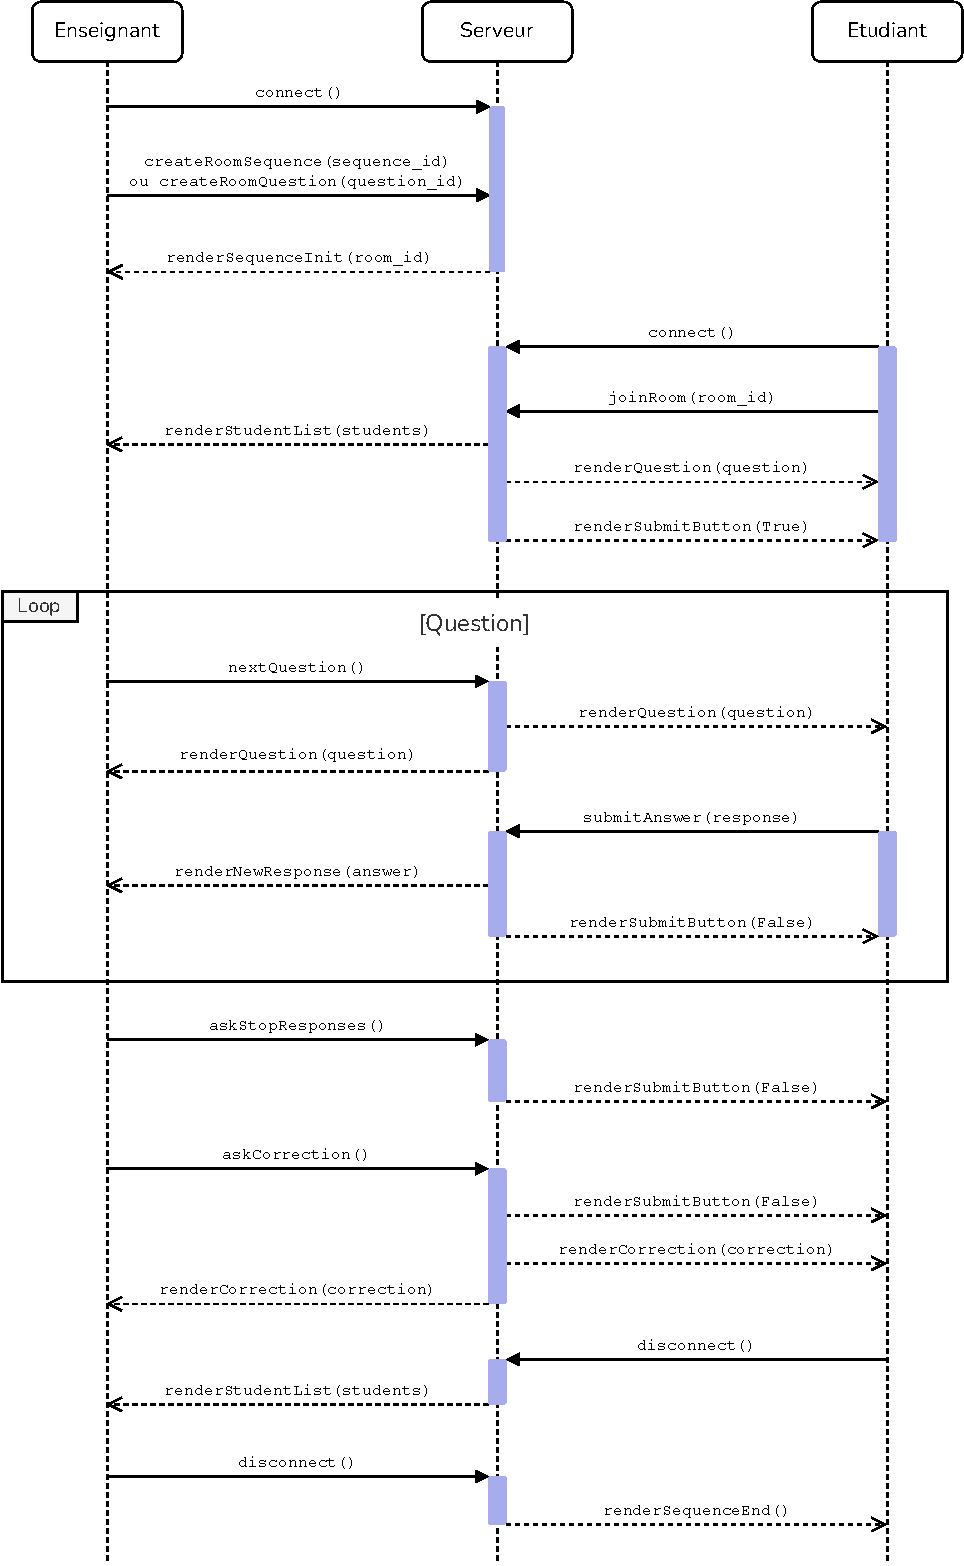
\includegraphics[width=13cm]{Diffusions.pdf}
\caption{Diagramme de séquence de la diffusion de quiz en direct avec WebSocket}
\label{fig:diffusions}
\end{figure}
\vspace{2mm}

Le diagramme de séquence présent dans la figure \ref{fig:diffusions} présente le diagramme de séquence qui décrit le fonctionnement des diffusions en direct sur notre site web. Ces diffusions utilisent un socket pour la communication en temps réel entre les enseignants et les étudiants.\\

Les enseignants peuvent créer une diffusion en émettant l'événement \texttt{createRoomSequence} ou \texttt{createRoomQuestion} en fonction du type de la diffusion. Cet événement déclenche la création d'une room Socket.IO et l'ajout de l'enseignant à cette dernière.\\

Les étudiants peuvent ensuite rejoindre la diffusion en entrant le code de la séquence, ce qui met à jour l'interface de l'enseignant en émettant l'événement \texttt{renderStudentList} à la room.\\

Les enseignants peuvent passer à la question suivante en émettant l'événement \texttt{nextQuestion} et les étudiants peuvent soumettre leur réponse avec \texttt{submitAnswer}. Les enseignants peuvent arrêter les réponses en émettant l'événement \texttt{askStopResponses} et demander la correction avec \texttt{askCorrection}.\\

Il est à noter que les enseignants ne sont pas obligés d'utiliser ces événements pour avancer dans la séquence et peuvent les utiliser dans l'ordre souhaité.

\vspace{5mm}
\subsection{Affichage des réponses en direct}
L'affichage des réponses en direct dans l'application est géré par une combinaison de deux composants : \texttt{StartSequenceView} et \texttt{RenderQuestion}.
Le composant \texttt{StartSequenceView} est le composant principal et est responsable de la gestion de la logique d'affichage des questions et des réponses en temps réel. 
Il utilise les composants \texttt{MultipleResponses} et \texttt{NumericResponses} pour afficher les réponses sous forme de graphique.\\

Les composant \texttt{NumericResponses} et \texttt{MultipleResponses} sont appelés en fonction du type de la question. Dans les deux cas les réponses numériques des étudiants sont affichées sur un graphique à barres, avec l'axe y représentant le nombre d'étudiants ayant donné une réponse spécifique, et l'axe x représentant les différentes réponses possibles. Le graphique est mis à jour en temps réel à mesure que les étudiants envoient leurs réponses. Comme demandé dans le cahier des charges, le site affiche maximum 5 barres (les 4 réponses les plus répondues et "Autres réponses").

\vspace{3mm}
\begin{figure}[H]
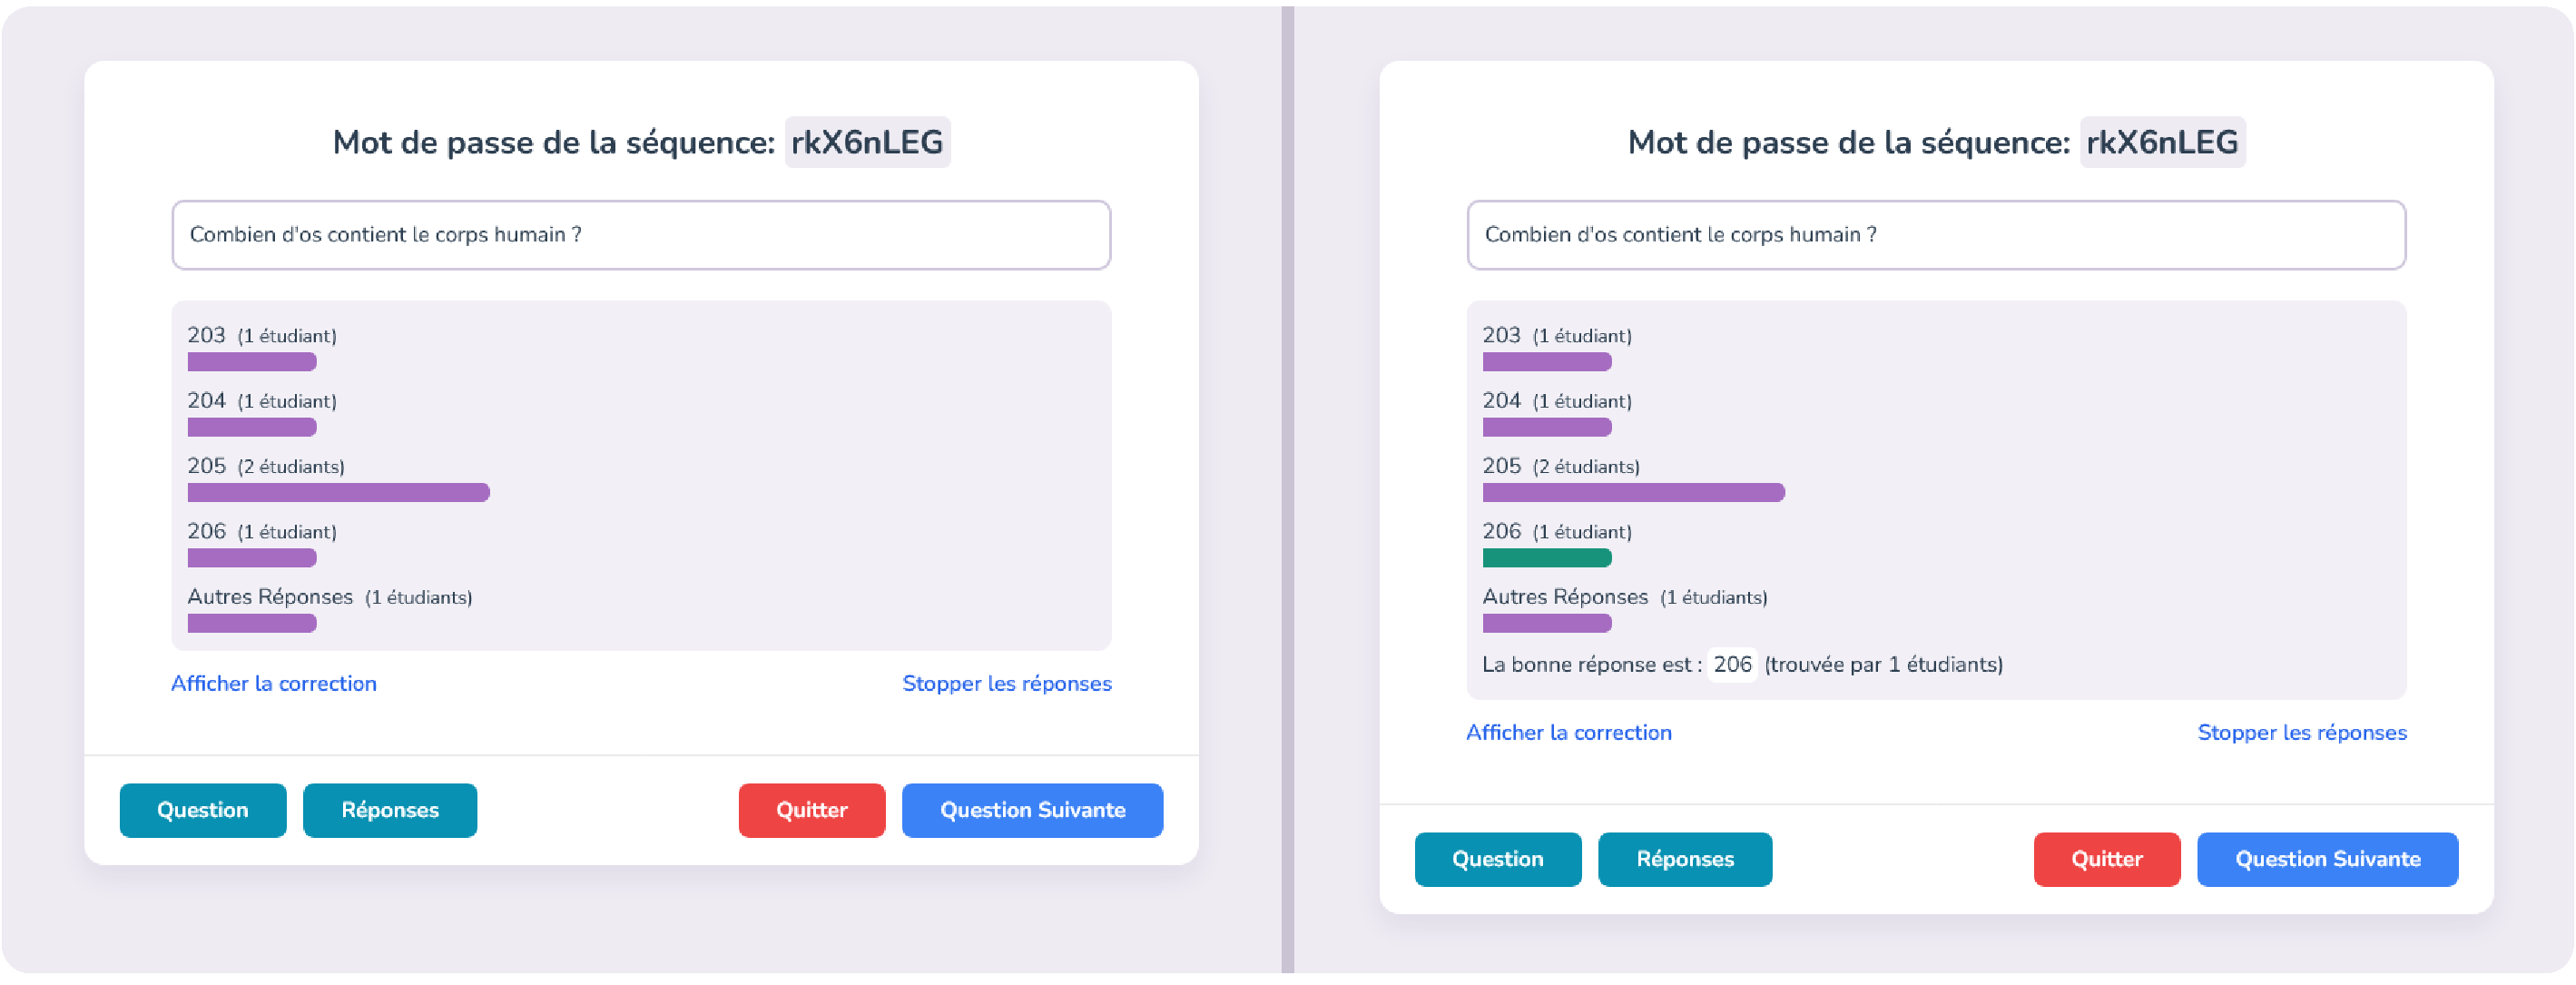
\includegraphics[width=\textwidth]{GraphiqueDiffusions.pdf}
\caption{Affichage des réponses en direct pendant la diffusion}
\end{figure}
\vspace{2mm}

\subsection{Authentification}
\begin{figure}[H]
\centering
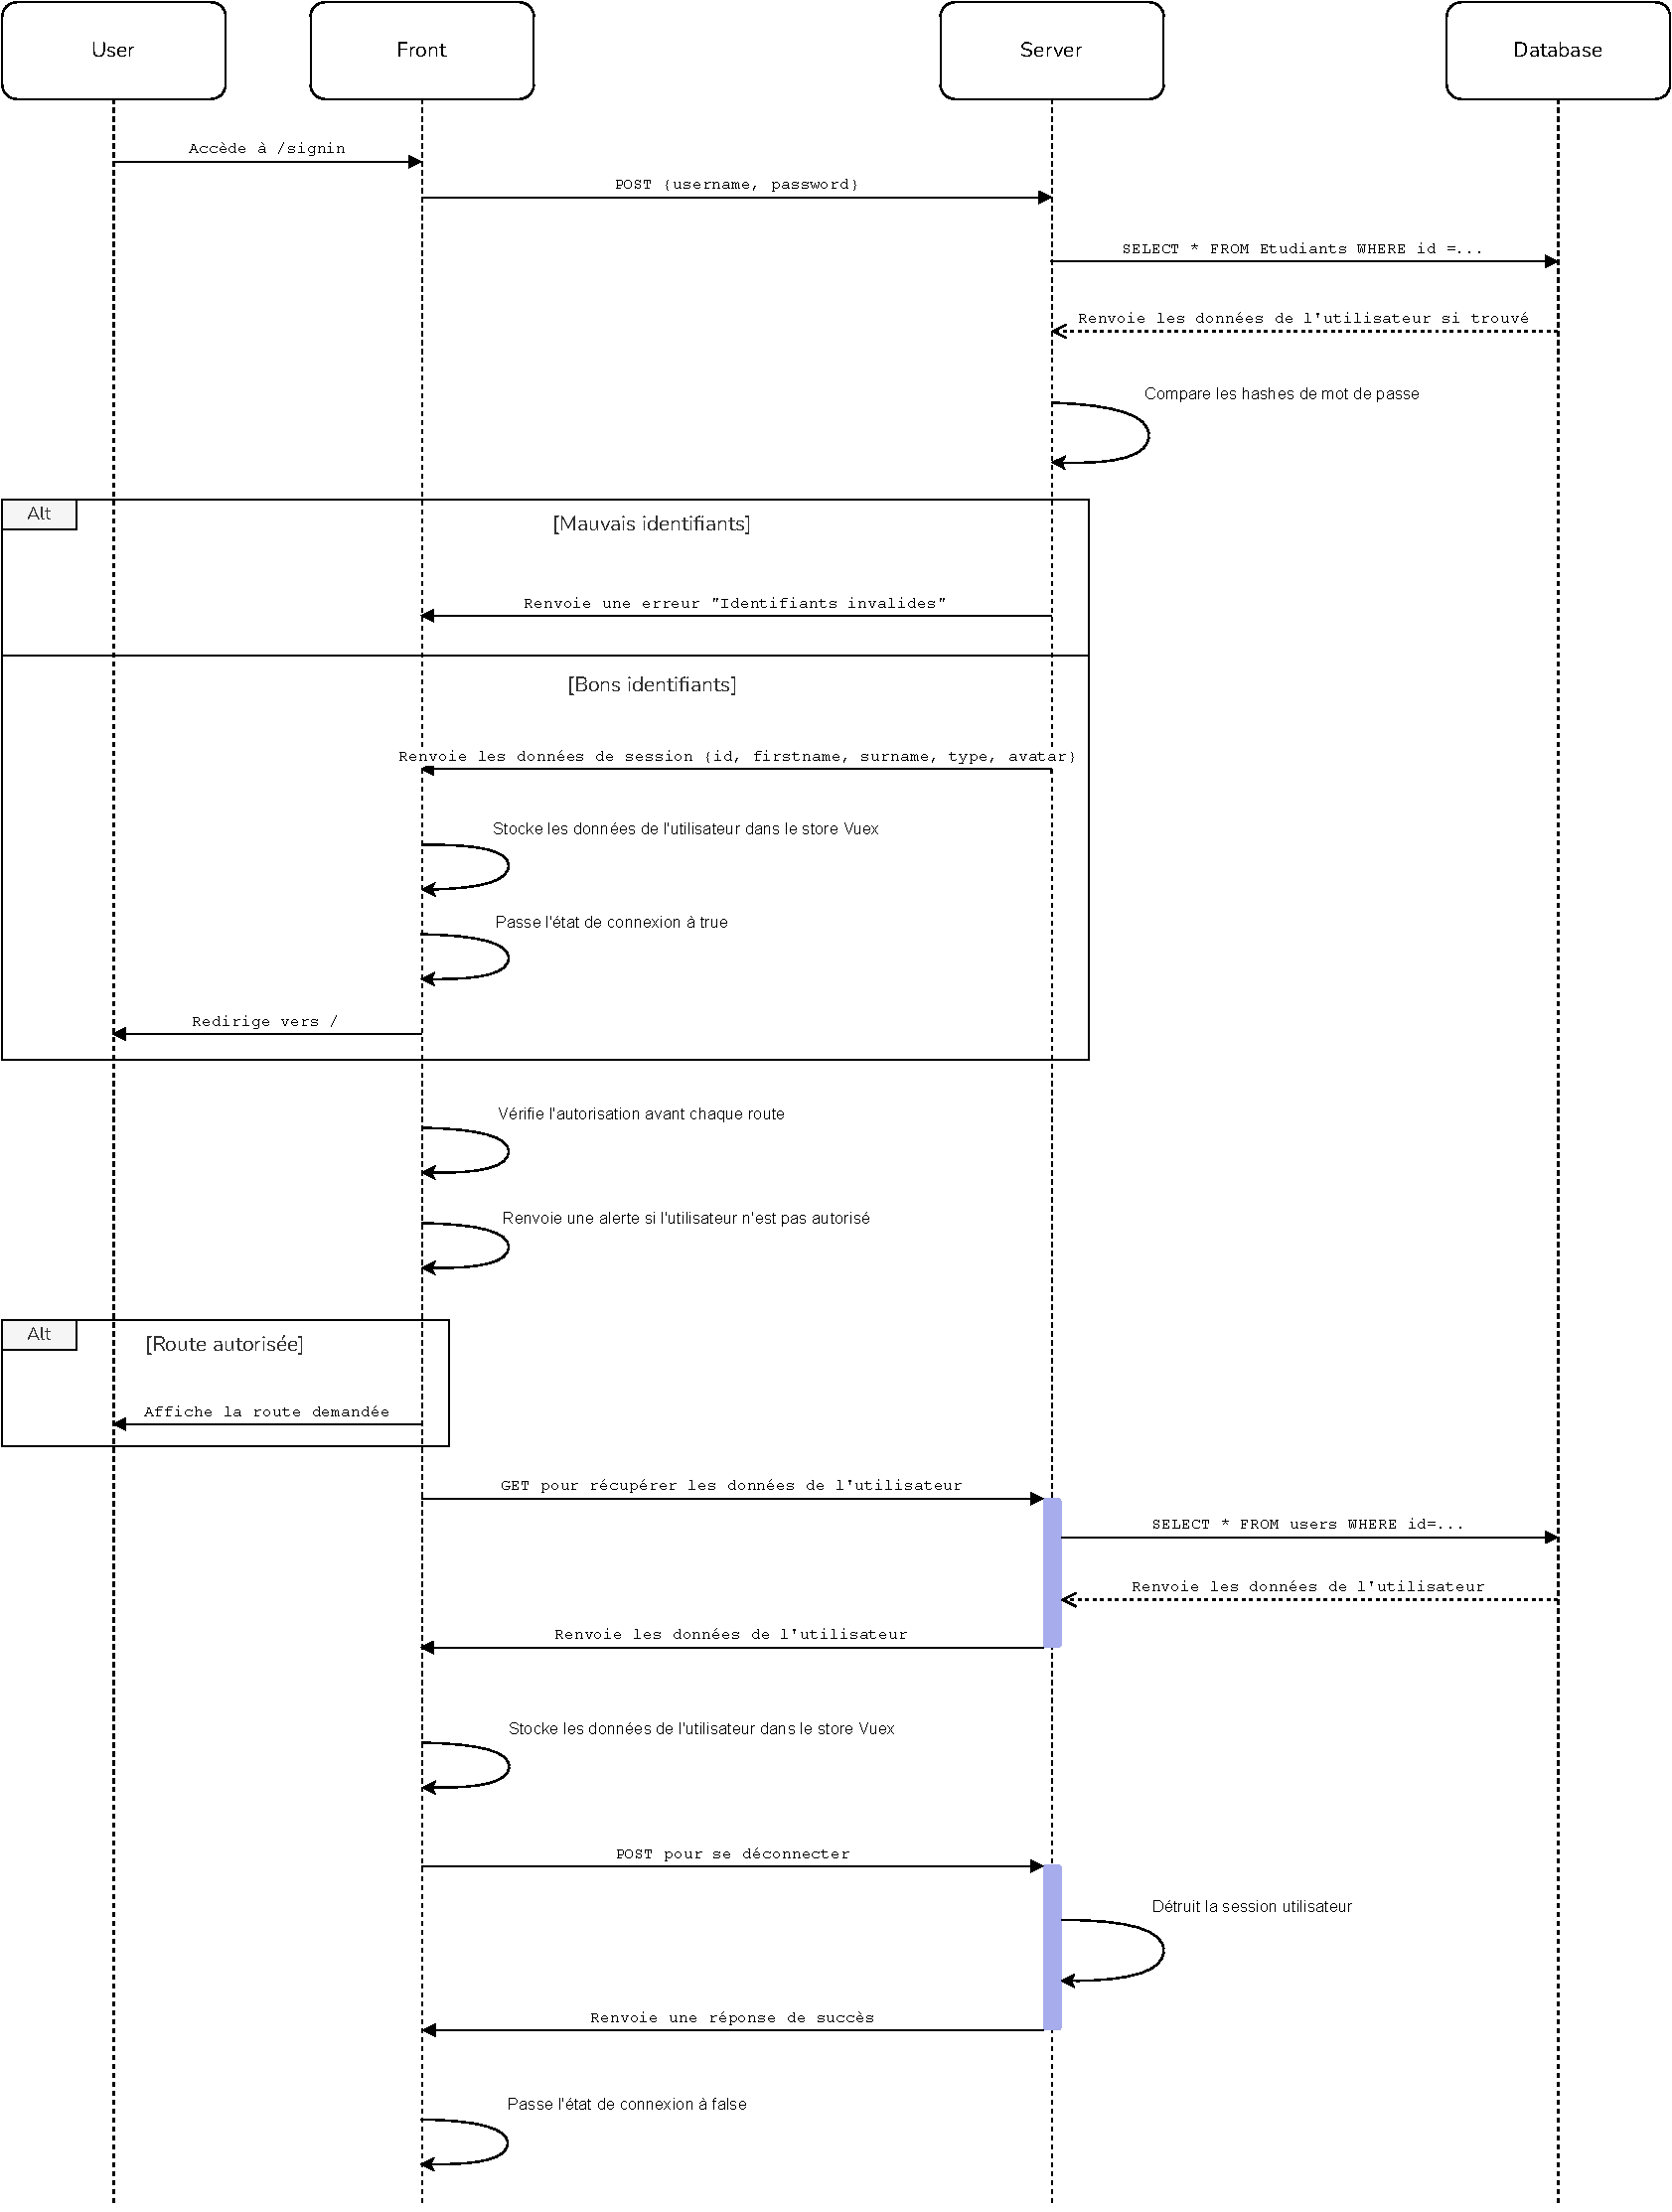
\includegraphics[width=\textwidth]{Authentification.pdf}
\caption{Diagramme de séquence pour l'authentification des étudiants}
\end{figure}

Le diagramme de séquence illustre le processus d'authentification pour les étudiants. Tout d'abord, l'étudiant entre ses identifiants sur la page de connexion. Ces informations sont alors envoyées au serveur pour vérification. Si les identifiants sont corrects, le serveur renvoie une réponse positive à l'étudiant, qui est alors redirigé vers la page d'accueil de l'application.\\

Pendant ce processus, le client (l'étudiant) interagit avec le serveur à travers des requêtes HTTP pour communiquer les informations nécessaires à l'authentification. Le serveur, quant à lui, vérifie les informations et répond avec un message indiquant si l'authentification a réussi ou échoué. Si l'authentification est réussie, le serveur envoie également les informations sur l'étudiant qui sont stockées dans la base de données.\\

De plus, le diagramme montre l'utilisation de deux technologies pour gérer l'état de l'application: le store Vuex et le routage. Le store Vuex permet de stocker les informations de l'utilisateur et de les rendre disponibles dans toute l'application. Le routage permet quant à lui de gérer la navigation entre les différentes pages de l'application et de vérifier si l'utilisateur est authentifié avant de lui donner accès à certaines pages.\\

En somme, ce diagramme de séquence représente de manière détaillée le processus d'authentification pour les étudiants dans l'application, tout en montrant les technologies utilisées pour gérer l'état de l'application.